\chapter{Sistema Quadrirotore}
Il capitolo è incentrato sulla descrizione del modello matematico del sistema quadricottero con le relative dinamiche, leggi di guida e leggi di controllo possibili da implementare.
\section{Modello matematico}
Il principio di funzionamento del quadrirotore è relativamente semplice nel suo complesso. Come accennato in precedenza la gestione dell'assetto è ottenuta attraverso l'azionamento differenziale dei rotori, montati su di una struttura rigida \cite{modelquad}.
Nel seguente elenco di manovre di base , viene preso come riferimento la figura \ref{fig:modello_quad}.
\begin{figure}
	\centering
	\begin{subfigure}{0.45\textwidth}
		\centering
		\includegraphics[width=1\textwidth]{SistemaQuadrirotore/Figure/drone_alto}
		\caption{Numerazione rotori}
		\label{fig:modello_quad}
	\end{subfigure}
	\hfill
	\begin{subfigure}{0.45\textwidth}
		\centering
		\includegraphics[width=1\textwidth]{SistemaQuadrirotore/Figure/drone_pitch}
		\caption{Variare l'angolo di beccheggio}
		\label{fig:modello_quad_pitch}
	\end{subfigure}
	\\
	\begin{subfigure}{0.45\textwidth}
		\centering
		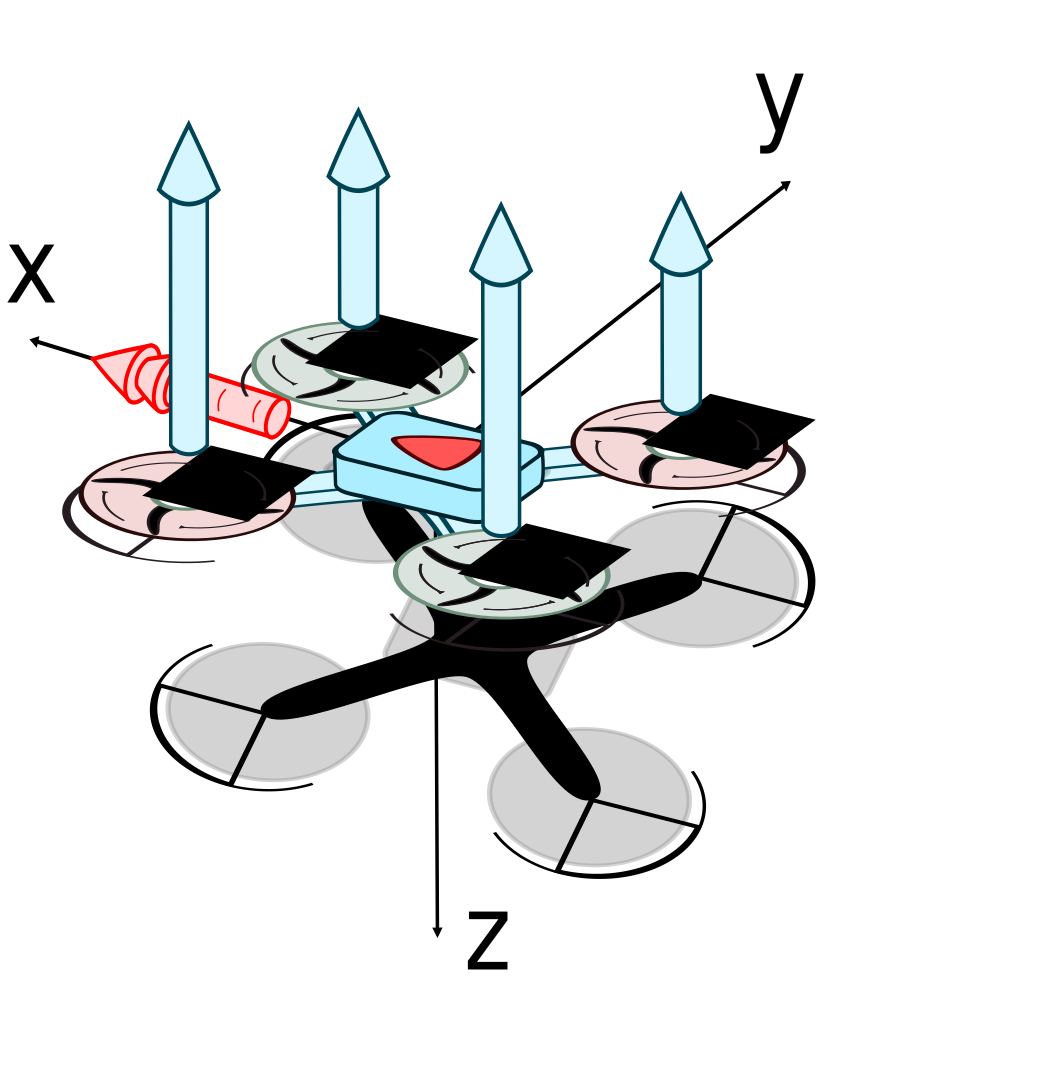
\includegraphics[width=1\textwidth]{SistemaQuadrirotore/Figure/drone_roll}
		\caption{Variare l'angolo di rollio}
		\label{fig:modello_quad_roll}
	\end{subfigure}
	\hfill
	\begin{subfigure}{0.45\textwidth}
		\centering
		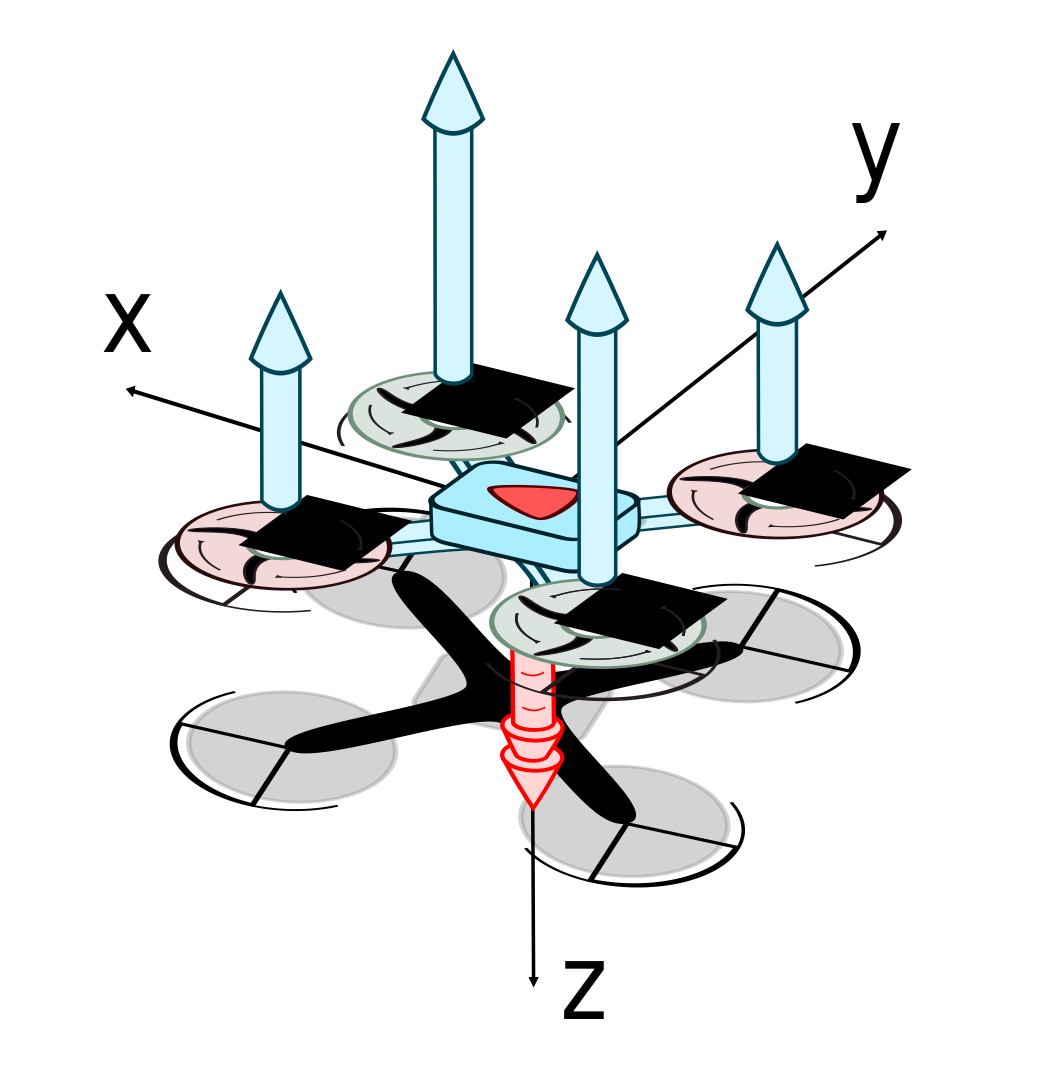
\includegraphics[width=1\textwidth]{SistemaQuadrirotore/Figure/drone_yaw}
		\caption{Variare l'angolo di imbardata}
		\label{fig:modello_quad_yaw}
	\end{subfigure}
	\caption{Schemi semplificati dell'azionamento del quadrirotore}
\end{figure}
\begin{itemize}
	\item \textbf{Comando di beccheggio : } una variazione di beccheggio positiva lungo l'asse y del corpo del drone avviene applicando maggiore forza ai rotori 2 e 3 rispetto ai 1 e 4, come mostrato nella figura \ref{fig:modello_quad_pitch}
	\item \textbf{Comando di rollio : } una variazione di vriazione dell'angolo di rollio positiva si ottiene modificando la velocità di azionamento dei rotori in modo simmetrico rispetto all'asse y del drone. come mostra la figura \ref{fig:modello_quad_roll} una variazione positiva si ottiene facendo ruotare i rotori 1 e 3 più lentamente dei rotori 2 e 4.
	\item \textbf{Comando di imbardata : } Questo comando è il meno efficace nel quadricottero in quando viene implementato attraverso un effetto secondario. Come si vede nella figura \ref{fig:modello_quad_yaw}, la rotazione dei rotori viene, mantendendo la portanza totale costante, distribuita in modo differente tra le pale che ruotano in modo orario e antiorario. Il comando di variazione positivo dell'angolo di imbardata si ottiene facendo ruotare più rapidamente i rotori 1 e 2 rispetto a 3 e 4.
	\item \textbf{Comando di spinta complessiva : } La variazione di quota avviene grazie a questo tipo di comando. Aumentando o diminuendo in modo identico la velocità di rotazione dei rotori è possibile equilibrare il peso, contrastato dalla portanza da essi generata. una portanza maggiore si traduce in una accelerazione verso l'alto, viceversa una diminuzione.
\end{itemize}
Attraverso questo funzionamento e l'utilizzo di un mixer, che ha lo scopo di mescolare i quattro tipi di azionamento visti, si può governare il velivolo modificandone la posizione nello spazio \cite{DesTestCarm}.
\subsubsection{Relazioni matematiche}
Esplicitando i sitemi di riferimento del corpo del drone e del riferimento terreste come in  \todo{Aggiungere figura riferimenti}figura, si può definire la matrice di rotazione $R$ espressa nella relazione \ref{eq:SistemaQuadrirotore_R}.
\[ 	c(\cdot)=\cos(\cdot)\ ,\  s(\cdot) = \sin(\cdot) \]
\begin{equation}
R=
	\begin{pmatrix}
	c(\psi)c(\theta)-s\phi)s(\psi)s(\theta) & -c(\phi)s(\psi) & c(\psi)s(\theta)+c(\theta)s(\theta)s(\psi) \\ 
	c(\theta) s(\psi)+c(\psi)s(\phi)s(\theta) & c(\phi)c(\psi) & s(\psi)s(\theta)-c(\psi)c(\theta)s(\phi) \\ 
	-c(\phi)s(\theta)	& s(\phi) & c(\phi)c(\theta)
	\end{pmatrix}
	\label{eq:SistemaQuadrirotore_R}
\end{equation}
\todo[inline]{I sistemi di riferimento e la rotazione da uno al altro}
\todo[inline]{Definizione degli operatori necessari a descrivere il modello base del drone}
\todo[inline]{Forze e momenti applicati nel modello di partenza}
\todo[inline]{Breve descrizione alle modifiche fatte al modello per applicazione su gazebo con rimando al capitolo specifico}